%\documentclass{sigchi}
\documentclass{article}


\usepackage{courier}
\usepackage{graphics} % for EPS, load graphicx instead
\begin{document}


%\title{Gismo: Document Exploration Through a Tool-Based Touch Screen Environment }
\title{Gismo: Graphical Interface for Searching with Multi-touch Objects}
\author{Prairie Rose Goodwin}
\date{}
\maketitle
\begin{abstract}
This project explores a new touch screen interface for interacting with data sets through a digital tool metaphor.  Research in psychology has shown that when we hold a tool, such as a hammer, our minds frame potential solutions around the affordances of the tool.  Additionally, metaphors have proven to be a powerful way to positively affect user experience, giving the user some expectations about how different objects behave.  Our system attempts to recreate the experience of using physical tools. Touch screens provide the ideal interaction style for this metaphor because they allow the user to be more physically engaged than a traditional point-and-click interaction. With the support of the James B. Hunt Library, we have created a work environment with life-size tools using a 40-inch PixelSense 2.0 touch screen table.  Our interface consists of two and a half dimensional representations of paperclips, pushpins, rulers, magnifying glasses, ``magic lenses", and sticky notes that can be used to manipulate database entries that appear as index cards scattered randomly on the table.  All objects on the screen have physical properties like center of mass, momentum, and friction to mimic the behavior of real objects on a table.  The tools are designed to let the user search and organize the data efficiently by taking advantage of spatial cognition and information visualizations.  Moreover, the user can leverage basic filtering queries by attaching ``filter tiles" to the tools that dictate the entries with which the tools will interact.  Our goal is to show that our system allows users to categorize data faster and more accurately than a comparable tabular interface.
\end{abstract}
\section{Keywords}
Information Visualization, Spatial Cognition, Spatial Memory, Document Management, Database Interface

\section{Introduction}	

Databases store vast amounts of data that people must interact with every day.  However, the interfaces that control databases have not changed significantly in the last thirty years.  Most are still command line-like  interfaces with a list of results that match the user's query.  Good interfaces will have a bar on the side to let you add additional filters to your search results.  There is no way to easily compare queries side by side, and it can be impossible to see trends within the list of results.

Desktop document management on the other hand has evolved considerably in the same amount of time.  Instead of working with a command line as seen in computers from the 70's and 80's, users now have files, folders, desktops, icons, thumbnails, shortcuts, and a myriad of other metaphors that improve usability and performance.   Gismo is a comprehensive graphical user interface for databases that pulls from many of the strengths of a desktop user interface. Instead of a desktop metaphor, Gismo uses a digital tool metaphor.

Tools are an integral piece of how humans interact with their physical environment.  When the analogy has been translated into a metaphor for software interfaces, it has been shown to have good usability, and users have adopted the metaphor with little difficulty.  However, these metaphors are only shallow representations of the full experience of using a physical tool.  Our program tries to incorporate as many aspects of tool use as possible.  We have chosen a technology that allows full movement of arms with a touch screen interface, and our digital representations of objects have naive physics that more closely mimic real world interactions.

In addition to a tool metaphor, Gismo draws on many strengths of the desktop user interface, such as using spatial memory to improve recall and organizational practices.  Databases are read dynamically into Gismo where the entries are translated into life size index cards that can then be moved around the screen.  The two and a half dimensional interface allows things to be focused, piled, pinned, and grouped.  Multi-touch interactions allow users to zoom, drag, and rotate as appropriate for the objects in the interface. 


The goal of this project was to create a graphical user interface that would transform database searches into a visual experience that leverages many of the cognitive benefits of tool use.

Our experiment was designed to test if a user could gain some understanding of the content of their data set without ever having seen it before.  We hypothesized that our system would allow users to more accurately determine the relatedness of an entry to a given subject, and that the user could do it faster than a traditional list-based interfaces that are common today.  

To do this we created a program that leveraged several different interactions that have shown to be beneficial to user performance:
\begin{itemize}
\item{Tools: Affordances of tools shape the users approach to problems put before them}
\item{Metaphors: simplify problems by framing them in a familiar context}
\item{Data visualizations: Provide context and can show patterns within the data set as a whole}
\item{Visual memory: improves recall of items}
\end{itemize}

In this paper, we describe the technology that we chose to use for this project (SUR40), the tool metaphor and how a user would utilize the tools, and the user study that we did to compare it to Mendeley.  We conclude with some discussion of why we felt our user trials did not yield positive results, and future work that we plan on doing for the next iteration of Gismo.


\section{Related Work} 
\subsection{Tool Metaphor}

GUI metaphors became popular because of their ability to reduce complicated tasks to a simpler structure.  %As cognitive tools defined by Hutchins \cite{Hutchins1995} and Norman \cite{Norman1991}, they have shown that they can be extremely powerful aids.  
The desktop metaphor, originally introduced by Xerox in the '70's, has become ubiquitous for personal computers.  Command line usability is notoriously difficult for beginners and non-technical users.  On the other hand, being able to interact with visual icons gives users an underlying model of the effect of their actions.  Giving users this mental mapping opened up computing to an entirely new demographic of people, and subsequently, the adoption of home computers skyrocketed.  

We explore a novel user interface with a tool metaphor for database searches.  Tool metaphors already exist in some conventional software environments.  Most notably, visual editing programs like Photoshop and Paint use analogs to real world objects like paint brushes and erasers to communicate functionality.  However, the metaphor is usually quite shallow, and beyond icon and task, bear little resemblance to the experience of using that tool.  This is important because there is a cognitive shift that occurs when using a physical tool in which the user starts to think of the tool as an extension of his or her body  \cite{Maravita2004}.  When we factor in the affordance of a tool, we realize that tool metaphors may have the ability to positively impact usability in ways that other metaphors may not.  

Direct manipulation interfaces provide a good environment to explore affordances in software \cite{Gaver1991} \cite{Norman1991}.  Users interact directly with objects on the screen instead of with menus or commands \cite{Hutchins1989} \cite{Shneiderman1992}, which are continuously represented with animation instead of appearing and disappearing as needed \cite{Shneiderman1992}.  Gentner argues that deeper metaphors that are more consistent with the physical world can improve learnability and usability of the system \cite{Gentner1996} and can be a good opportunity for the user to become familiar with the system \cite{Fischer1994}.  


\subsection{Spatial Cognition}
Previous research has shown the cognitive benefits of being able to organize items spatially \cite{Agarawala2006} \cite{Robertson1998}. Robertson et. al made a two and a half dimensional interface called DataMountain for bookmarking websites that showed dramatic improvement in efficiency and error over the built in text-based system.  DataMountain's design is very similar to ours so we will discuss their work in depth throughout the paper.    
	
	Numerous studies have compared graphical environment and textual environments.  Sebrechts et. al most notably did a formal evaluation of text-based, 2-D, and 3-D interfaces \cite{Sebrechts1999}.  They found that the 2-D interface had the best performance in both user satisfaction and performance with modern input devices.  They varied the input devices, and found that they made a significant impact on the usability of the interface. The more closely the input method matched the visualization on the screen, the more usable the system.  This result lends support that touch may be the best interaction technique for direct manipulation interfaces such as ours.  

\subsection{Touch}
Touch screens have become popular in recent years, but they are often a step backwards in usability \cite{Norman2010}.  Gesture-based interfaces have many of the drawbacks of a command line interface: commands can be hard to remember, impossible to explore, and hard to debug.  There are no visual cues for what gestures the system will recognize, and there is not a standard set of gestures for all functionality.   Some work has been done to standardize gestures to make them more intuitive \cite{North2009}, but adoption of standards continues to be a problem with few exceptions like pinch to zoom.  

	Other work suggests that multi-touch interfaces may have usability gains similar to command-line interfaces for expert users \cite{Forlines2007} \cite{Tan2002} \cite{North2009}. The biggest efficiency gain comes in target selection, which is the majority of screen interaction \cite{Forlines2007}.  The nearly unlimited number of available gestures allows a lot more to be done in a smaller amount of space and time.  
	
	Tabletop touch screens have a significantly different interaction experience than smaller screens.  Consequently, some of the conventions used on other devices have not translated well.  On larger touch screens, users benefited from direct touch input over mouse which is a more active experience \cite{Kristensson2008}.  This may seem counter intuitive because of the larger amount of movement required to reach the entire screen. However, the kinesthetic signals (muscle memory) that are associated with embodied movements have been shown to improve spatial recall by 19\% in an experiment in document retrieval \cite{Tan2002}. This may also have impacts on overall the overall usability of large screens.


\subsection{Document Management}

So much of what we do with computers is dependent on being able to find pertinent information.  Many systems have focused on how to keep personal documents organized in a desktop interface for quick retrieval with positive results \cite{Agarawala2006} \cite{Foo2007:ECDL} \cite{Foo2007:ICADL}. However, scaling the interfaces to be able to handle large amounts of data continues to be an unsolved problem \cite{Whittaker2001}.

Some interfaces have tried different visualizations to put as much information on the screen as possible \cite{Newman2010} \cite{Nowell1996} \cite{Shneiderman2000} \cite{Yost2006}.  These types of interfaces try to find some way to group things together into topics \cite{Newman2010}, but a lot of information is lost when this is done \cite{Nowell1996}.  Because our understanding of natural language processing is imperfect, the algorithms doing the modeling can make imperfect decisions.  This leads to documents being miscategorized (and therefore overlooked), or making decisions that are not obvious to the user.  GUI's benefits are significantly reduced when the user's mental model breaks down, which causes confusion.  

Trying to use spatial relationships to display different kinds of information seems to be a better solution \cite{Bier2005} \cite{Foo2007:ECDL} \cite{Foo2007:ICADL} \cite{Mothe1998}.   Bier et. al used the x,y position of a document to communicate the value different attributes, allowing multiple metadata to be easily seen at the same time \cite{Bier2005}.  %Foo et. al, took several different graphical visualizations (e.g. List view, tree view, map view, etc.) and compared them to see which one users preferred. \cite{Foo2007:ECDL} 
Similarly, INQUERY was a system that grouped results into row and column clusters based on related data \cite{Mothe1998}.  Ultimately, all of these still only provide surface-level information.  This can make it more difficult to look at different aspects of the data, since these interfaces cannot be modified to organize information based on search criteria.
 
%\cite{Newman2010}
%This paper explores visualizations of document collections, which we call topic maps. Our topic maps are based on a topic model of the document collection, where the topic model is used to determine the semantic content of each document. Using two collections of search results, we show how topic maps reveal the semantic structure of a collection and visually communicate the diversity of content in the collection. We describe techniques for assessing the validity and accuracy of topic maps, and discuss the challenge of producing useful two-dimensional maps of documents.

%While not explored in this paper, we have the opportunity to use many visualization techniques to improve the usability and interpretability of our topic maps, beyond simple color coding by a single topic. We often have other attributes or metadata (such as authors, citation links and subject headings) that can enhance= topic maps, using any combination of color, shape, size and text annotations.

%One conclusion from this work is that local topic maps (which dynamically show a few dozen closely related documents) may be more accurate. While topics are a useful way to organize an entire collection, producing a static global topic map of the collection may have limited value for exploring the collection. Therefore local topic maps may ultimately be more useful for better understanding and navigating local structure in a collection.


%\cite{Nowell1996}
%A digital library of computer science literature, Envision provides powerful information visualization by displaying search results as a matrix of icons, with layout semantics under user control. Envision’s Graphic View interacts with an Item Summary Window giving users access to bibliographic information, and XMosaic provides access to complete bibliographic information, abstracts, and full content. While many visualization interfaces for information retrieval systems depict ranked query-document similarity, Envision graphically presents a variety of document characteristics and supports an extensive range of user tasks. Formative usability evaluation results show great user satisfaction with Envision’s style of presentation and the document characteristics visualized.

%For the
%two benchmark subtasks using the Graphic View,
%participants made no errors, asked no questions, and all
%required less time than expected to complete the benchmark
%tasks — to our delight, surpassing the performance of an
%Envision designer!


%\cite{schraefel2002}
%Hunter Gatherer is an interface that lets Web users carry out three main tasks: (1) collect components from within Web pages; (2) represent those components in a collection; (3) edit those component collections. Our research shows that while the practice of making collections of content from within Web pages is common, it is not frequent, due in large part to poor interaction support in existing tools. We engaged with users in task analysis as well as iterative design reviews in order to understand the interaction issues that are part of within-Web-page collection making and to design an interaction that would support that process.We report here on that design development, as well as on the evaluations of the tool that evolved from that process, and the future work stemming from these results, in which our critical question is: what happens to users perceptions and expectations of web-based information (their web-based information management practices) when they can treat this information as harvestable, recontextualizable data, rather than as fixed pages?


%\cite{Shneiderman2000}
%Digital library search results are usually shown as a textual list, with 10-20 items per page. Viewing several thousand search results at once on a two-dimensional display with continuous variables is a promising alternative. Since these displays can overwhelm some users, we created a simplified two-dimensional display that uses categorical and hierarchical axes, called hieraxes. Users appreciate the meaningful and limited number of terms on each hieraxis. At each grid point of the display we show a cluster of color-coded dots or a bar chart. Users see the entire result set and can then click on labels to move down a level in the hierarchy. Handling broad hierarchies and arranging for imposed hierarchies led to additional design innovations. We applied hieraxes to a digital video library of science topics used by middle school teachers, a legal information system, and a technical library using the ACM Computing Classification System. Feedback from usability testing with 32 subjects revealed strengths and weaknesses.
%\cite{Yost2006}
%Larger, higher resolution displays can be used to increase the scalability of information visualizations. But just how much can scalability increase using larger displays before hitting human perceptual or cognitive limits? Are the same visualization techniques that are good on a single monitor also the techniques that are best when they are scaled up using large, high-resolution displays? To answer these questions we performed a controlled experiment on user performance time, accuracy, and subjective workload when scaling up data quantity with different space-time-attribute visualizations using a large, tiled display. Twelve college students used small multiples, embedded bar matrices, and embedded time-series graphs either on a two megapixel (Mp) display or with data scaled up using a thirty-two Mp tiled display. Participants performed various overview and detail tasks on geospatially-referenced multidimensional time-series data. Results showed that current designs are perceptually scalable because they result in a decrease in task completion time when normalized per number of data attributes along with no decrease in accuracy. It appears that, for the visualizations selected for this study, the relative comparison between designs is generally consistent between display sizes. However, results also suggest that encoding is more important on a smaller display while spatial grouping is more important on a larger display. Some suggestions for designers are provided based on our experience designing visualizations for large displays. Index Terms—Information visualization, large displays, empirical evaluation.
\section{Gismo}


\begin{figure}[b!]
\centering
\scalebox{.239}
{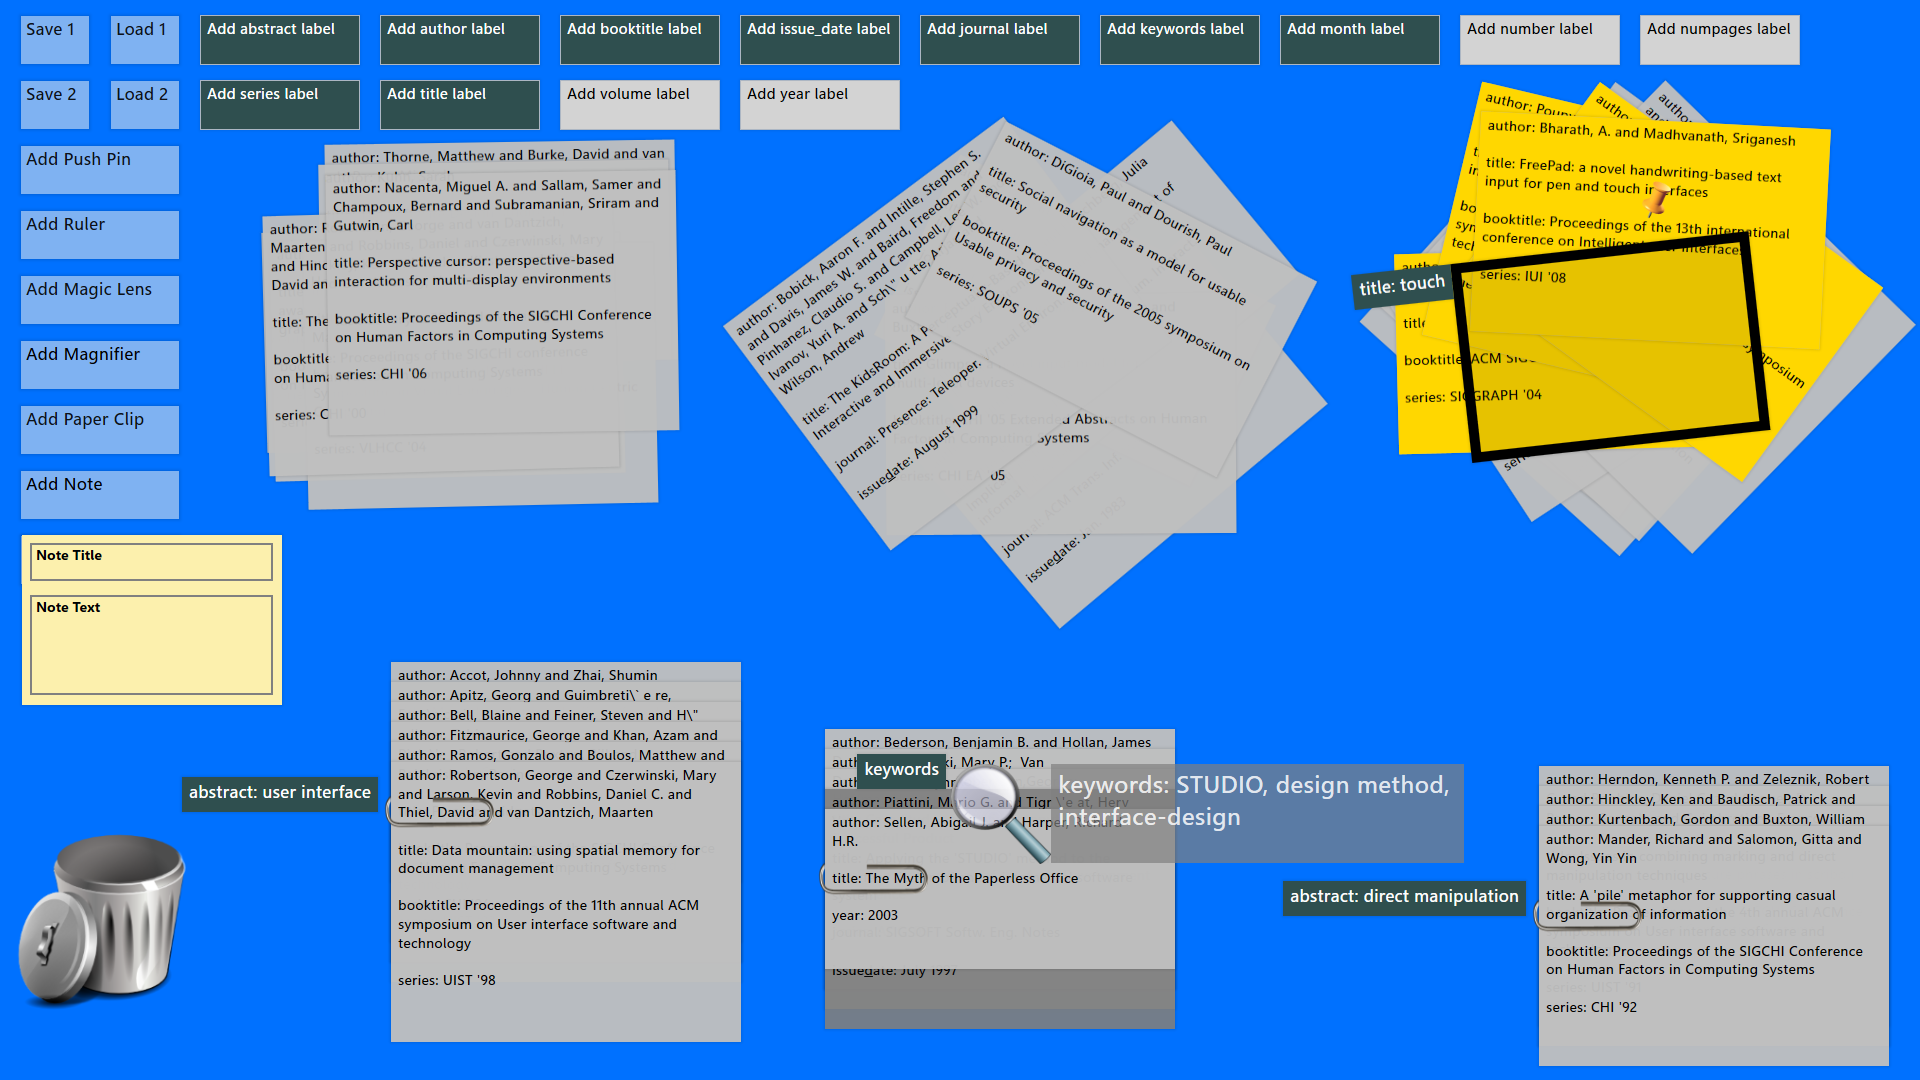
\includegraphics{HabilisScreenShot.png}}
\caption{Screenshot of Gismo using various tools.}
\label{Fig:screenshot}
\end{figure}


We propose a novel way to display and organize information visually through the metaphor of physical tools. Tool-use in the physical world generally includes an object in the operator's hand and broad motions to perform an action. We have extended these concepts to digital tools by implementing a program on the Microsoft PixelSense 2.0 that lets the user select (pick-up) tools on the screen and perform motions that mimic physical tool usage. Users interact with objects on the screen by direct manipulation with an established set of interaction mechanism.  

This program would be used to search and organize information stored in a database.  After getting an initial body of entries to search, each entry will appear as individual tiles with properties of naive physics that can be moved around the screen by touch. 



\subsection{Software Design Decisions}

We felt that it was important that Gismo's use case was not too narrowly focused.  We wanted it to be flexible enough to be able to be data independent and be used by both beginners and experts.  It's backend has three layers.  The lowest layer is where the data is stored independently in a relational database, bibTex, or other format. The middle layer consists of a parser that converts that data from it's original form into the internal representation of Entries and Filters.  The highest layer is the interface where the user interacts with the data. 

\subsection*{Data}

Since we were pulling from a pool of graduate students for our user study, we decided to have our data focus on research publications, pulled mostly from the ACM, IEEE, and Springer digital libraries.  The easiest way to store our data was in bibTex.  The data was copied directly from the website, and then the abstracts were added to the entries manually for our purposes.  This was the only time that a human modified the data in any way.

When the user saves his or her session, it is saved into a bibTex file, with the added attributes of x, y, orientation, and z-index.  When the session is reloaded, the parser recognizes these attributes and sets the corresponding values in the internal representation rather than reading them into the list of attributes.  


\subsection*{Parser}

The middle layer needs to be written specifically for whatever kind of database you are using to store your data.  We realize that this is a major trade-off to not have the program working out of the box, but abstracting the data out of the interface was the best choice for both performance and flexibility. 

The middle layer performs two steps:
\begin{enumerate}
\item{Create a list of all possible attributes and their data type.}
\item{Read in the data and create a card for each item in the database.} 
\end{enumerate}


The current parser is for bibTex and is optimized slightly for our data.  Even though, almost every entry had a URL where the full text could be found, we had to have the parser ignore it, because C\# was stalling on the slashes.  After loading it in once, we decided to have it ignore a couple of other attributes (``location", ``articleno") that only appeared in one entry and would therefore not be useful for searching.

%Parsing out bibTex is easy for a computer to do.  Every 

The starting screen of the interface has buttons at the top of the screen for each unique attribute that appears in the database.  The background of the button is determined by the attributes data type, so the parser has to determine these things before loading.  The database is read into the program dynamically at each start-up and  

\begin{figure}[t!]
\centering
\scalebox{.5085}
{\includegraphics{bibTexToEntry.png}}
\caption{This figure goes through how the data looks in each later.  The data layer consists of plain text in bibTex form.  The middle layer creates an attribute HashMap that is used as the backend for the Entry that appears on the screen.}
\label{Fig:bibTexToEntry}
\end{figure}



%Gismo is built to be flexible for different kinds of information.  The database is read into the program dynamically at start up.  A button is populated for each unique attribute at the top of the screen and is labeled with its name.  During this process, the program tries to infer what data type is associated with each attribute.  Gismo is robust enough to be able to handle many common data types such as numbers, dates, strings, list of numbers, and list of strings.  Each data type has a hard-coded color that is associated with it.  If it detects a non-string data type, it will change the background of the button and the associated FilterTiles to that color.  Additionally, the FilterTiles will be able to accept the comparison functions associated with that data type.  If Gismo cannot detect a data type, then the type defaults to a string.  When each entry is created, it saves the attributes and corresponding values to a HashMap to be accessed in queries later.  
%
%The current version of Gismo is optimized to read from bibTex for our experiment.  The process to change what kind of database it reads from requires two steps to get the data into the program's representation:  read in the names of all attributes, and read every row and convert it into a HashMap.  As long as there is a way to do these two things, that database will be compatible with Gismo.

\subsection{Save States}
Gismo includes two save states.  You can switch between two configurations of data for comparative purposes.  The tools do not change when a save state is loaded.  This is done to maintain object permanence and to facilitate using the same queries on either configuration.  

\subsection{Filter Tiles}
The name of each attribute or column header is shown on buttons that generate a label when pressed. These labels specify search criteria and can be attached to the tools to determine the items with which the tool will interact. For example, if the attribute is a string, the user can specify a query string that will be used in a ``contains" search within that attribute. If the attribute is a number, the user can use any of the comparison functions available such as greater than, less than, etc. 

Example: Assume that your dataset is a collection of research papers with the attributes: 
\begin{itemize}
\item{(String) Title }
\item{(String) Author }
\item{(Date) DatePublished}
\item{(List$<$String$>$) Keywords}
\item{(int) pages}

\end{itemize}

If you are looking for a paper on computer vision published in the last five years that is between five and ten pages long, you could create the query labels:
\begin{itemize}
\item Pages: $>$ 5
\item Pages: $<$ 10
\item Date: $>$ 2009
\item Keywords: ``Computer Vision"
\end{itemize}

Once created, the filter tile can be attached to tools by intersecting the two objects.  To detach, a long touch will remove the filter tile from the screen.

\subsection{Gismo Tools}
The focus of this project was searching, so the tools that were useful for that task can accept filters. However, for other tasks, we found it was more useful to have tools that were consistent for all entries.  These tools were used for modifying entries based on their location rather than their content.  Therefore, filters were disabled for the following tools.
\subsection*{Push Pin}
The pushpin is used to ``save" entries.  Once pinned, the entry is immobilized and no other tool can modify that entry.  Entries can be thrown under a pin to create a messy pile with casual organization.  
\subsection*{Ruler}
The ruler can push entries around the screen and organize them visually by aligning them horizontally or vertically.  This state is somewhere in between a tidy pile and a messy pile \cite{Agarawala2006} as it does not afford browsing.  However, it unmistakably shows you entries that are categorized together.  
\subsection*{Sticky Note}
Sticky Notes attach directly to entries and look similar to a filter with a different background color.  Once attached, the note will display the title, but the user can tap it once to switch to the body and title of the note.
\subsection*{Trash Can}
The trashcan removes any unwanted entries or tools.  Just like in a Desktop GUI, the user can drag the item to the trash can, and it will disappear from the screen.  
\subsection{Gismo Filter Tools}
The following tools can be modified by attaching filter tiles.  Once attached, the tool will only interact with the entries that match the tile's query.  
\subsection*{Magic Lens}
The magic lens is a window that highlights entries that match your query.  Additionally, the lens will pop the results to the front of the interface so that no results are hidden.  The main functionality lets you see the results of queries without modifying the entries.  As a result, you can explore several queries side by side or consecutively before making decisions about your next action.    
\subsection*{Magnifier}
The magnifier lets the user view any attribute of an entry.  To activate the magnifier, you must drag a filter tile to the magnifier.  Instead of creating a query, the corresponding data of that attribute will be displayed in a pop-up next to the magnifier.  The magnifier will accept any number of filter tiles, and the attribute will be displayed below the last one.  
\subsection*{Paper Clip}
Paper clips create organized piles, or ``tidy piles".  If no filters are attached, the paper clip will pick up everything.  If a filter tile is added, it will drop any entries that do not match the query.   With this tool, the user can easily separate the entries in which you are interested from those that you are not.

\begin{figure}[t]
\centering
\scalebox{.623}
{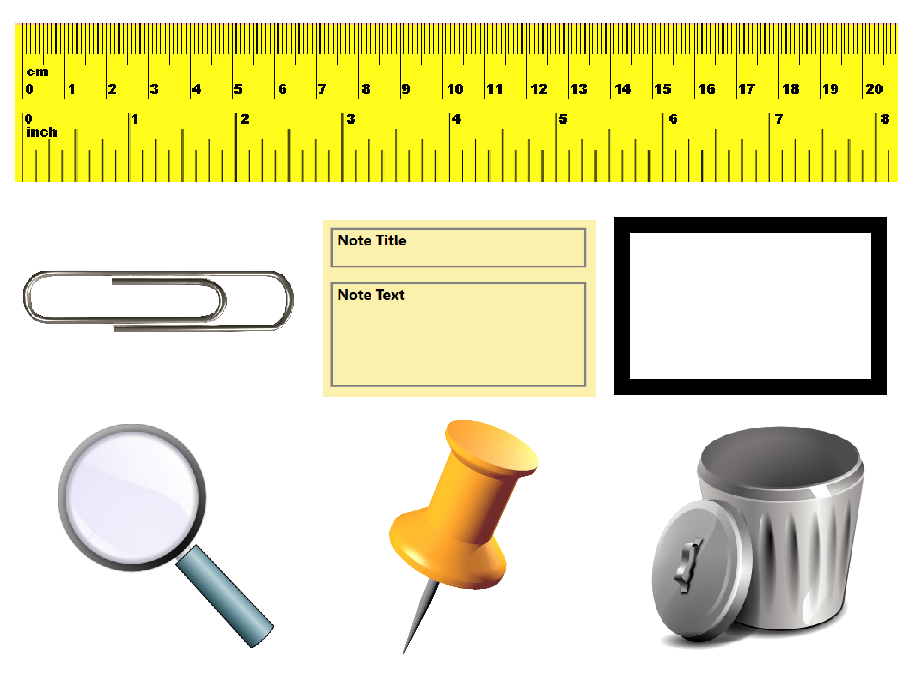
\includegraphics{ToolsFigure.png}}
\caption{Images used for digital tools.  From Top to bottom, and left to right: Ruler, paperclip, sticky note, magic lens, magnifier, push pin, and trash can.}  
\end{figure} 


\subsection{Gismo Interaction Design}
The buttons that are initially placed on the screen to populate the tools are not movable, scalable, or rotatable.  They can be activated by a quick or long touch and have no other interactions.  

The other UI Elements are sub-classed from a ScatterViewItem, a PixelSense 2.0 specific object class, and all have the same interaction properties.  All elements have physical properties like center of mass, momentum, and friction to mimic the behavior of real objects on a table.  You can drag them around using one finger, but dragging with two fingers  disables the tool's interactions so that you could drag it to where you would like to use it.  Additionally, you can do a two finger rotation as you would expect, and a one finger rotation around the center of mass.  Objects can be flicked across the screen, bouncing when it reaches the edge of the screen (a fullscreen ScatterView object).  All objects, including filter tiles and notes, are activated by intersecting the borders of the items.  Once a filter tile or note has been attached to its target, it can be removed with a long touch (1.5 seconds).  

\subsection{Hardware and Developer Tools}

\begin{figure}[t!]
\centering
\scalebox{1}
{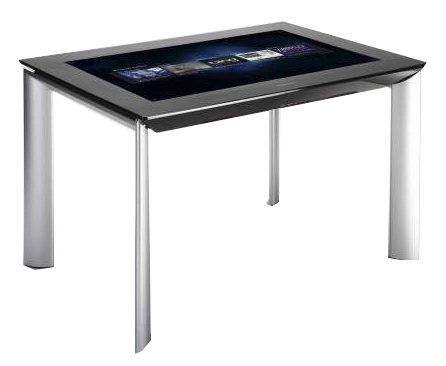
\includegraphics{SUR40.jpg}}
\caption{SUR40 Touchscreen Table}
\label{Fig:table}
\end{figure}

The PixelSense 2.0 developer packages for the SUR40 have a lot of positives that made it attractive for this project.  The developer tools have parent classes ScatterView and ScatterViewItem that gave objects physical properties.  When touched, a shadow was activated to give the illusion of the item being picked up.  ScatterViewItems have built in multi-touch gestures, such as pinch to scale, dragging, and rotations. Additionally, they had inertia, momentum, and a center of mass that allows users to do a one finger rotation as well.  The ScatterView is optimized for ScatterViewItems creating an environment in which they can exist.  ScatterViews have well defined edges that ScatterViewItems cannot cross, instead bouncing off the edge when thrown.  When a ScatterViewItem is places on it, its rotation and placement is random so to encourage users to stand on any side of the table.  These objects, combined with the C\# wpf framework, minimized the amount of physics that we had to program by hand.

The touch screen table was designed in a way that allows a single user could reach any part of the screen without barring access to multiple users simultaneously.  The touchscreen is not capacitive.  Each pixel also contains an IR Sensor and an RGB Sensor.  The table relies on the distance of your hand from the screen as read by the IR sensor to determine whether or not you are touching it.  Additionally, the RGB sensor allows the table can recognize ``Microsoft Tags" which are simpler QR codes that can be used for object recognition.  

The fact that the table uses IR sensors expands the realm of interactions.  For example, digital art could be painted with an actual paint brush.  For traditional computing, it gives the user the ``hover" state, where the user targets a UI element without activating it, for a third interaction state.  However, it also reduces its usability since the IR sensor has a lot more noise than a capacitive touch screen.  

\section{User Study}

Our work with Gismo pulls heavily from the concepts established in Robertson et. al \cite{Robertson1998}.  Their system, Data Mountain, focuses on organizing bookmarks from the world wide web instead of database entries, but the tasks are similar enough cognitively that we decided to structure our user study similarly to theirs.  

Robertson used a between users study where each participant was placed in one of three groups.  Everyone in each group used either Internet Explorer 4 (IE4), Data Mountain 1, or Data Mountain 2 (a revised version of Data Mountain 1 based on user feedback).  Participants were given 100 web pages to store in whatever organizational structure that they wanted.  In the second half of the experiment they had to retrieve the web pages within a given amount of time.  They measured four variables: retrieval time, incorrect retrievals before finding the correct page, failed trials, and a user evaluation.  

We decided that we could do a similar study to evaluate Gismo.  Both programs use spatial cognition to organize a data set and both programs are designed to give users an understanding of content based on attributes.  Instead of simply retrieving a given entry, we asked users to make objective categorizations to test if they actually understood what the data set contained.  Although there are many similarities between Data Mountain and Gismo, there are some significant differences between our user studies that are more suited to our domain tasks.   

The goal of our experiment was to see if a user could gain some understanding of the content of their dataset without ever having seen it before.  We designed our experiment to test two hypotheses:  

\begin{enumerate}
\item{Users will be able to more accurately determine relatedness of an entry to a given subject using Gismo than with Mendeley.}
\item{Performance time using Gismo will be lower than the performance time of using Mendeley.}
\end{enumerate}

	We were originally planning for fifteen to twenty participants, but our preliminary feedback showed definitively negative results.  As a result, we decided to cut the user trials short after eight participants.  If we had gone forward, we would have completed a full power analysis to ensure that we had enough participants for an effective sample size \cite{Lenth2001}.  
	

%Gismo went through several iterations with pilot studies to determine the usability of new features.  




\subsection{Methods}
\subsection*{Subjects}
	Eight Computer Science graduate students between the ages of 22 to 26 from various research specialties participated in this study.  No one had previous experience using Gismo or the SUR40, while six out of eight had no previous experience with Mendeley. All subjects were male with  normal or corrected-to-normal vision with no other known disabilities. 
\subsection*{Equipment}
	Gismo was run on the Samsung SUR40 40-inch touch screen table with no external hardware.  Users were forced to use only touch interactions with a virtual onscreen keyboard. Mendeley was run on a Sony Flip-PC touch screen convertible laptop.  However, no user chose to utilize the touch interactions of the laptop, and instead used a wireless mouse and build in keyboard.  
	
\subsection*{Procedure}

	This experiment was a comparative study between Gismo and Mendeley.  To test which system was better for organizing documents into categories, users were asked to identify citations of a source paper.  We chose to use Bumptop \cite{Agarawala2006}
	as our source paper because it has many sources that neatly divide into several subjects.  The authors also released a seven minute video that gives a detailed overview of all of the features and novel designs without mentioning their sources.   
	
	Bumptop has forty-one sources that encompass six subjects: advantages of a pile metaphor, stylus interactions, spatial organization, realism, browsing techniques, naive physics, and animation.  Dataset one encompassed twenty-one papers covering pile metaphors, stylus interactions, and spatial organization.  The remaining twenty papers went into dataset two.  Distractor papers were added from mobile and touchscreen research until each dataset had a total of thirty-seven papers.  The subjects were then asked to identify which papers were related to Bumptop.  The datasets were alternated between Gismo and Mendeley to overcome any performance bias of the data.  The trials were timed, and at the end they were asked to answer a short survey.  
	
\section{Results}

Unfortunately, the IR technology that this table used to determine touch did not work as well as we had hoped.  In fact, this model was discontinued within a year and a half of its release because of significant hardware performance problems.  When sitting in front of the table, it is as likely to read the users wrist as a touch as his or her finger.  When it recognized a ``blob" where your palm could be seen, it would register circa 50 events in and around that area.  If there were significant smudges on the table, that could throw off what was happening where your hand was because it saw a multi-touch gesture.  The most significant problem however, was that the calibration was so sensitive that if the lighting changed at all from when you calibrated it, the table would not function correctly.  This meant that it could not be placed in any room with natural light.  It took us several months to figure out this problem, not realizing that the time of day or the weather could have such a significant impact on the table's usability.  

Once we got the table into a windowless room, we were able to improve many of the problems programmatically within Gismo, but the on screen keyboard continued to be a major source of frustration for the users.  Five of the eight participants mentioned that they had shied away from using the tools because the keyboard registered so many incorrect events, making it impossible to type.  Beyond the keyboard, sometimes an event triggered by a wrist would make something fly across the screen which would break the user's concentration.  The hardware faults caused the usability of Gismo to suffer greatly, but the magnitude of the problem was not apparent until user trials had begun.  
      
\subsection*{Performance Time}


The performance time of Gismo ended up being slower than Mendeley.  This can be explained by a few things.  First, two users did not utilize the tools at all and instead just read the attributes off of the card.  Second, the hardware event misfires as described above had a tendency to break the user's train of thought, and they had to compensate by taking time to get back to where they were before the event had fired.  Third, none of the users had any familiarity with Gismo before the trials.  Since they were learning the system while using it, there is the possibility that performance time would improve over time. 


Robertson et. al  \cite{Robertson1998} also looked at this metric.  The completion times are used directly in their analysis of variance, without adjustments for non-normality.  Therefore, we also assume a normal distribution for performance time.



\begin{figure}[h!]
\centering
\scalebox{1}
{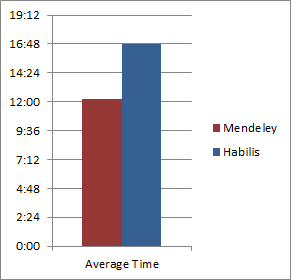
\includegraphics{AverageTime.png}}
\caption{Average Time for completion}
\label{Fig:timeChart}
\end{figure}


A single factor analysis of variance (ANOVA) was performed on the performance time of the data grouped within subject. Mendeley takes less time to complete the task than Gismo with $F=3.25$ and $p < 0.06$.  Doing a t-test on the same data found $t=-3.18$ and $p<0.01$. 




\subsection*{Number of Incorrect Categorizations}

We had hypothesized that users could more accurately categorize the data with Gismo than with Mendeley.  However, our trials showed that the opposite was true.  We think that this was a combination of an unfamiliar system combined with an under utilization of the tools available.  No one used the sticky note, six did not use the ruler, and some tools were used once and then never again.  Most interactions were with the paperclip, push pin, and magic lens.    

Mendeley and Gismo performed equally twice, but otherwise Mendeley provided better results.  A Single Factor ANOVA was performed on the number of correctly categorized papers with a statistically reliable main effect where $F=6.4$ and $p<0.03$

\begin{figure}[ht!]
\centering
\scalebox{1}
{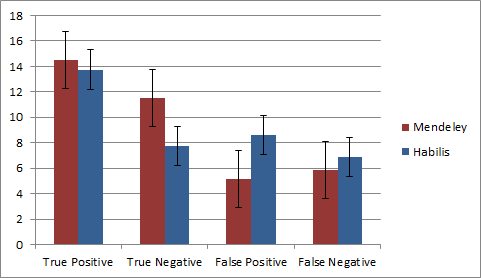
\includegraphics{BarChartSquare.png}}
\caption{SUR40 Touchscreen Table}
\label{Fig:barChart}
\end{figure}



\subsection*{Questionnaire}
Once finished, the users answered three questions about their experience.  
%%RESULTS
	\begin{enumerate}
	\item Which system did you prefer? Why?
	\item Did you see any topic clusters?  If so, what topics?
	\item What features were you looking for but didn't see in Gismo?
	\end{enumerate}

The first question asks about user preference, the second asks about cognitive benefits, and the third is  about usability and feature visibility.  

	Three users said that they preferred Gismo to Mendeley, and a fourth said that he would if the ghost events of the table could be fixed.  With nearly half enjoying the experience despite the system bugs, there is potential to raise this number if all of the hardware problems can be fixed.  
	
	Many of the design principles that went into this project were to help visualize overall trends in the data.  All of the users identified a mobile theme in dataset two, while two users identified touch based themes while on the table for dataset one.    These are the distractor themes.  Six of the eight users identified a physics theme, but the rest of the subjects that were recorded were not listed by more than one user.  
	
	The last question yielded the most interesting results.  By asking this question, we were able to determine which features were not immediately visible to the user.  For example, three users said that they would have liked a way to read the abstract of the papers.  The magnifier will bring up the abstract to read for just this purpose, but these individuals never found this functionality, even if they had used the magnifier for other purposes.  Another person mentioned that they wished that there was a way to organize the entries into a sorted list.  All paperclips automatically alphabetize the pile based on the first attribute, in this case author.  The other suggestions were minor: have the papers snap to the middle of the push pin; change the active area of an entry; cut down on the clutter of the buttons at the top.  These suggestions imply that the users are already thinking around the affordances of the interface.  After only a small amount of time with Gismo, no one asked for anything that would be difficult to integrate into the existing interface.  


\section{Discussion \& Future Work}
Unfortunately, our user study did not demonstrate that Gismo was an effective alternative to Mendeley.  We felt that this result was due in large part to the hardware rather than the design.  A more accurate touch screen would decrease user frustration and may encourage users to explore the interface more.  

One of the most common feedback that we received was that the ``messy" initial state was a little overwhelming.  If we could somehow group the papers to begin with, it would give the user some place to start.  The next iteration of this program will use intelligent topic modeling (Latent Dirichlet Allocation) to provide the user with piles at start up.  There will be a simple interface that will allow the user to decide which attributes they want to use for the topic modeling and to vary the parameters to their needs.  

Another point of improvements will be on the scalability of the interface.  Like most GUI's there is a tradeoff of visual benefits vs screen space.  Although performance doesn't degrade very quickly, after about 200 entries, Gismo becomes unwieldy simply because there is not enough space in which to work with the entries efficiently.  

In summary, we have created a novel touch screen database interface for exploring datasets visually through a tool metaphor.  Our contribution derives from utilizing technology to create an interface that has benefits over traditional computing.  We believe that Gismo has been a successful cognitive tool that reduces large problems into a simpler task, and with some more fine tuning, we are confident that it will show concrete benefits over list based interfaces.  




\bibliographystyle{plain}
%\bibliographystyle{acm-sigchi}
\bibliography{890}{}
\end{document}
